\documentclass[tikz,border=3mm]{standalone}
\usetikzlibrary{matrix,positioning,fit,backgrounds}
\begin{document}
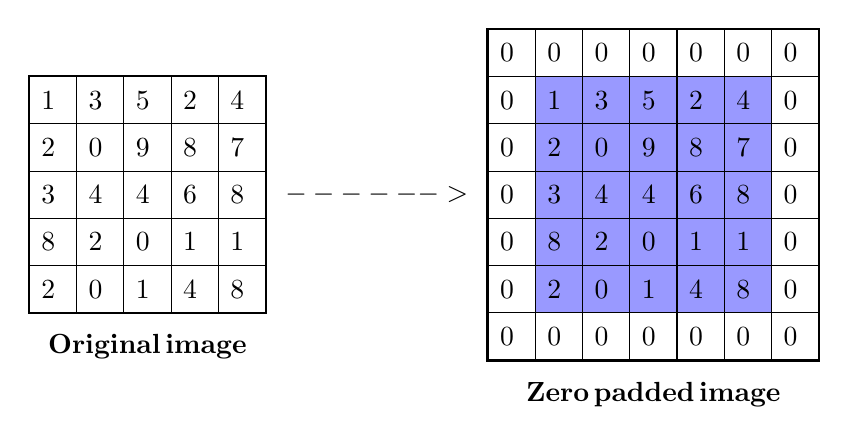
\begin{tikzpicture}[mmat/.style={matrix of nodes,
	column sep=-\pgflinewidth/2,
   row sep=-\pgflinewidth/2,
   cells={nodes={draw,inner sep=2pt,thin}},draw=#1,thick,inner sep=0pt},
  nodes in empty cells,
  nodes={
  	minimum size=.6cm,
  	anchor=center,
  	align=center,
  	},
   mmat/.default=black,
   node distance=0.3em]
 \matrix[mmat](mat1){
         1 & 3 & 5 & 2 & 4  \\ 
         2 & 0 & 9 & 8 & 7   \\ 
         3 & 4 & 4 & 6 & 8   \\ 
         8 & 2 & 0 & 1 & 1   \\ 
         2 & 0 & 1 & 4 & 8   \\ 
         };
 \node [below= of mat1.south] (i) {$\bf Original\,image$};
 \node[right=of mat1] (eq) {$------>$};  
 \matrix[mmat, right=of eq](mat2){
 	 0 	& 0 & 0 & 0 & 0 & 0 & 0 \\
 	 0 	& 1 & 3 & 5 & 2 & 4 & 0  \\ 
 	 0 	& 2 & 0 & 9 & 8 & 7 & 0  \\ 
 	 0  & 3 & 4 & 4 & 6 & 8 & 0  \\ 
 	 0 	& 8 & 2 & 0 & 1 & 1 & 0  \\ 
 	 0  & 2 & 0 & 1 & 4 & 8 & 0  \\
 	 0  & 0 & 0 & 0 & 0 & 0 & 0 \\ 
 };
\node [below= of mat2.south] (i) {$\bf Zero\,padded\,image$};
\scoped[on background layer]
{
	\node[fill=blue!40, fit=(mat2-2-2)(mat2-6-6),inner sep=0pt] {};
}
 

 
\end{tikzpicture}
\end{document}
